\subsection{Basic Theory of Sintering}\label{subsec:basic-theory}

The following elaborations on the basic theory of sintering are based on standard literature for the topic. Some notable textbooks are those of \textcite{German1996, German2014}, \textcite{Geguzin1973}, \textcite{Kang2005} and \textcite{Exner1978}.

This work concentrates on solid state sintering, which means that there are no other than solid phases present in the system (exept the surrounding atmosphere).
Liquid phase sintering, where the material partially melts to assist closing pores, shall not be regarded.
Therefore, the term sintering shall always refer to solid state sintering from here on.

Sintering in general is a process, where powder material is densified and strengthened by thermal treatment at elevated temperatures.
The process is mainly driven by reduction of the energy stored in the system microstural features, such as grain boundaries, surfaces and other crystal defects.
These features are transformed by diffusional flows of material to reach a state of lower energy.
In this process, energy is dissipated, so it is an irreversible process.

\begin{figure}
	\centering
	% 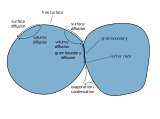
\includegraphics{img/introduction/state_of_the_art/diffusion_mechanisms}
	\caption{Schematic Overview of Diffusion Mechanisms Observed in Sintering Processes}
	\label{fig:introduction/state_of_the_art/diffusion_mechanisms}
\end{figure}

In common sintering processes the following diffusion mechanisms may occur, but their importance depends on powder geometry, process conditions and material properties.
The place and usual direction of their occurence is visualized in \autoref{fig:introduction/state_of_the_art/diffusion_mechanisms}.

\begin{description}
	\item[Volume Diffusion] Diffusion in the bulk material mediated by vacancies. Usually one of the slowest mechanisms and often neglegible.
	\item[Surface Diffusion] Diffusion along free surfaces (interfaces with surrounding atmosphere or vacuum). Much faster than volume diffusion.
	\item[Grain Boundary Diffusion] Diffusion along grain boundaries (solid-solid interfaces). Usually slower than surface diffusion but faster than volume diffusion.
	\item[Evaporation/Condensation] Evaporation of atoms to the gas phase and condensation at another point. Fast transport through the gas phase, but usually occurs only at very high temperatures or with very volatile substances.
\end{description}

Sintering is usually divided in three stages:

\begin{description}
	\item[Initial/Early Stage] Creation of initial contact. Major diffusion along surfaces to the sinter neck (triple points of surfaces and grain boundary). Rapid increase of neck size but low shrinkage.
	\item[Intermediate Stage] Porosity is still open and connected. Major diffusion along grain boundaries to the pores. Removal of substance at grain boundaries leeds to large shrinkage.
	\item[Final/Late Stage] Mainly closed porosity, gas pressure in pores may affect sintering. Still mainly grain boundary, but also volume diffusion. Slow progress in shrinkage and densification.
\end{description}

\subsubsection{Mathematical Description of Diffusion}

The classic description of diffusional processes is done by Fick's laws \textcite{Fick1855} based on the heat conduction laws by \textcite{Fourier1888}.
\autoref{eq:fick-first} shows Fick's first law for description of the diffusional flux $\Flux$ for the one-dimensional case.
It proposes a linear relationship between the concentration gradient and the flux.
For the concentration here the vacancy concentration $\VacancyConcentration$ is taken, as we assume only one diffusing species.
The flux of vacancies equals the negative flux of atoms.

\begin{equation}
	\Flux = - \DiffusionCoefficient \frac{\Deriv\VacancyConcentration}{\Deriv\X}
	\label{eq:fick-first}
\end{equation}

The diffusion coefficient heavily varies with temperature.
Its temperature dependence is usually described by an Arrhenius-type equation as in \autoref{eq:diffusion-coefficient-arrhenius} with a pre-exponential factor $\DiffusionCoefficient_0$ and the activation energy $\ActivationEnergy$. 

\begin{equation}
  \DiffusionCoefficient = \DiffusionCoefficient_0 \exp \left( -\frac{\ActivationEnergy}{\GasConstant\Temperature} \right)
	\label{eq:diffusion-coefficient-arrhenius}
\end{equation}

The local vacancy concentration as driving force of the diffusion, however, depends on the thermal equilibrium vacancy concentration $\VacancyConcentration^\Standard$ and the local chemical potential $\Potential$ as in \autoref{eq:vacancy-concentration}. 

\begin{equation}
  \VacancyConcentration = \VacancyConcentration^\Standard \left( 1 - \frac{\Potential - \Potential^\Standard}{\GasConstant\Temperature} \right)
  \label{eq:vacancy-concentration}  
\end{equation}

The main factor influencing the chemical potential in the regarded sintering processes are stresses, especially stresses originating from curved surfaces or interfaces (also known as surface tensions). The local chemical potential by a stress $\Stress$ is given as in \autoref{eq:potential-stress} with the molar volume $\MolarVolume$. 

\begin{equation}
  \Potential = \Potential^\Standard + \Stress \MolarVolume
  \label{eq:potential-stress}
\end{equation}

The stress by a curved surface is given as in \autoref{eq:stress-surface-curvature} with the surface resp.\ interface energy $\InterfaceEnergy$ and the curvature $\Curvature$.

\begin{equation}
  \Stress = \InterfaceEnergy \Curvature
  \label{eq:stress-surface-curvature}
\end{equation}

Other stresses present affect the progress of sintering nevertheless. 
The reason for pressure assisted sintering can directly be seen from these equations, since the applied pressure drives the diffusion from the inner of the grain boundaries to the necks.

